\documentclass {scrartcl}
\usepackage[a4paper, left=2.5cm, right=2.5cm, top=2.5cm, bottom=3cm]{geometry}
\usepackage[english]{babel} % wegen deutschen Umlauten
\usepackage[utf8]{inputenc}
\usepackage{color}
\usepackage{listings}
\usepackage{fancyhdr}
\usepackage{graphicx}		% Einbinden von Bildern
\usepackage{ulem}				% Einbinden von Bildern
\usepackage{multicol} 	% Spalten
\usepackage{tipa} 			% Sonderzeichen wie | (pipe)
\usepackage{textcomp} 	% spitze klammern
\usepackage{rotating}
\usepackage{hyperref}   % hyperlinks
\usepackage{pdfpages}
\usepackage{subcaption}
\usepackage{float}


%%%%%%%%%%%%%%%%%%%%%%%%%%%%%%%%%
% Adapt every excercise
%%%%%%%%%%%%%%%%%%%%%%%%%%%%%%%%%
\newcommand{\VersionNr}{1.0}
\newcommand{\Subject}{Carrera Protocol VHDL Design}
\newcommand{\Name}{Lukas Rappel}
\newcommand{\Number}{S1510567014}


% Kopf-/Fußzeile
\pagestyle{fancy} %eigener Seitenstil

\fancyhf{} %alle Kopf- und Fußzeilenfelder bereinigen
\fancyhead[L]{Version \VersionNr} %Kopfzeile links
\fancyhead[C]{FH Hagenberg \\ \Subject} %zentrierte Kopfzeile
\fancyhead[R]{\Name\\ \Number} %Kopfzeile rechts
\renewcommand{\headrulewidth}{0.4pt} %obere Trennlinie
\fancyfoot[C] {-{\thepage}-} %Seitennummer
\renewcommand{\footrulewidth}{0.4pt} %untere Trennlinie
% C++ Source code
\definecolor{dkgreen}{rgb}{0,0.6,0}
\definecolor{gray}{rgb}{0.5,0.5,0.5}
\definecolor{mauve}{rgb}{0.58,0,0.82}
\setlength{\headheight}{26pt}
%%%%%%%%%%%%%%%%%%%%%%%% listings settings %%%%%%%%%%%%%%%%%%%%%%%%%%%%%%%
\lstset{ %
language=C++,                % choose the language of the code
basicstyle=\footnotesize\ttfamily,       % the size of the fonts that are used for the code
numbers=left,                   % where to put the line-numbers
numberstyle=\footnotesize,      % the size of the fonts that are used for the line-numbers
stepnumber=1,                   % the step between two line-numbers. If it is 1 each line will be numbered
numbersep=5pt,                  % how far the line-numbers are from the code
backgroundcolor=\color{white},  % choose the background color. You must add \usepackage{color}
showspaces=false,               % show spaces adding particular underscores
showstringspaces=false,         % underline spaces within strings
showtabs=false,                 % show tabs within strings adding particular underscores
frame=single,           				% adds a frame around the code
tabsize=4,          						% sets default tabsize to 2 spaces
captionpos=b,           				% sets the caption-position to bottom
breaklines=true,        				% sets automatic line breaking
breakatwhitespace=false,    		% sets if automatic breaks should only happen at whitespace
keywordstyle=\color{blue},      % keyword style
commentstyle=\color{dkgreen},   % comment style
stringstyle=\color{mauve}       % string literal style
%escapeinside={\%*}{*)}         % if you want to add a comment within your code
}
%%%%%%%%%%%%%%%%%%%%%%%% hyperlinks settings %%%%%%%%%%%%%%%%%%%%%%%%%%%%%%%
\hypersetup{colorlinks,
pdfstartview = FitH,
bookmarksopen = true,
bookmarksnumbered = true,
linkcolor = black,
plainpages = false,
hypertexnames = false,
citecolor = black
}

\lstset{
literate={ö}{{\"o}}1
{ä}{{\"a}}1
{ü}{{\"u}}1
{ß}{{\ss}}1
{é}{{\'e}}1,
inputencoding=ansinew,
extendedchars=true
}

\title {\Subject \\ \VersionNr}
\author {\Name (\Number)}
\date {\today}

\begin {document}
\maketitle
\tableofcontents
\newpage
%%%%%%%%%%%%%%%%%%%%%%%%%%%%%%%%%%%%%%%%%%%%%%%%%%
\section{Overview}
\begin{figure}[h]
	\centering
		\includegraphics{./Blockdiagramm.PNG}
	\caption{Overview CarreraProtocol unit}
	\label{fig:SocGhostCar_IP}
\end{figure}

\subsection{Interface}

\begin{table}[h]
	\centering
		\begin{tabular}{|r|c|l|}
		\hline
		\textbf{Signalname} & \textbf{Width} & \textbf{Description} \\
		\hline		
		\hline
		iDataAsync & 1 & Positive rail signal (Manchester encoded); asynchronous \\
		\hline
		oID & 32 & Telegram ID, generated by internal counter.\\
		oData & 16 & Telegram content as 16-Bit value.\\
		oBitLen & 4 & Bit length of last successfully received telegram.\\
		\hline
		oNewData & 1 & Status information: new data available.\\
		oError & 1 & Status information: error detected (auto reset).\\
		\hline
		iClk & 1 & System Clock.\\
		inResetAsync & 1 & Asynchronous inverted Reset input.\\
		\hline
		\end{tabular}
	\caption{VHDL Entity Interface}
	\label{tab:VHDLEntityInterface}
\end{table}

\subsection{External parts}
The carrera rail signal has a nominal value of 18V. In order to adapt the signal level to fpga's logic level of 3{,}3V, a voltage divider is used.

$$ \frac{U_{fpga}}{U_{rail}} = \frac{R_1}{R_1+R_2} = C = 0,18333$$

$$ R_2 = R_1 \cdot \frac{(1-C)}{C} = R_1 \cdot 4{,}45455 $$
$$ R_1 = R_2 \cdot \frac{C}{(1-C)} = R_2 \cdot 0{,}22449$$

\subsection{QSYS Interface}
Memory mapped slave interface
\subsection{Register Mapping}
\begin{table}[h]
	\centering
		\begin{tabular}{|r|c|l|}
				\hline
		offset & width & description \\
		\hline
		\hline
		0 & 32 & Telegram ID \\
		\hline
		1 & 32 & Telegram data\\
		\hline
		2 & 32 & Bit 0-3: Telegram bit length \\
		  & & Bit 8: new data available\\
			& & Bit 9: (bus) error detected (auto reset)\\
		\hline	
		\end{tabular}
	\caption{Register Mapping}
	\label{tab:RegisterMapping}
\end{table}

\section{Functional description}
\subsection{Protocol}
The Carrera Protocol is described on \href{http://www.slotbaer.de/index.php/carrera-digital-124-132/12-d132-d124-daten-protokoll}{www.slotbaer.de}.

The protocol contains 10 datawords with different bit length: 
\begin{table}[h]
	\centering
		\begin{tabular}{|r|c|l|}
				\hline
			dataword & width & content \\
		\hline
		\hline
Programmierdatenwort & 12 & 1 W0 W1 W2 W3 P0 P1 P2 0 0 R0 R1 R2\\
		\hline
PaceUndGhostCardatenwort & 9 & 1 1 1 1 KFR TK FR NH PC TA \\
		\hline
Aktivdatenwort & 7 & 1 R0 R1 R2 R3 R4 R5 IE \\
		\hline
Reglerdatenwort 0 & 9 & 1 R2 R1 R0 SW G3 G2 G1 G0 TA \\
		\hline
Reglerdatenwort 4 & 9 & 1 R2 R1 R0 SW G3 G2 G1 G0 TA \\
		\hline
Reglerdatenwort 1 & 9 & 1 R2 R1 R0 SW G3 G2 G1 G0 TA \\
		\hline
Reglerdatenwort 5 & 9 & 1 R2 R1 R0 SW G3 G2 G1 G0 TA \\
		\hline
Reglerdatenwort 2 & 9 & 1 R2 R1 R0 SW G3 G2 G1 G0 TA \\
		\hline
Aktivdatenwort &  7 &1 R0 R1 R2 R3 R4 R5 IE \\
		\hline
Reglerdatenwort 3 & 9 &1 R2 R1 R0 SW G3 G2 G1 G0 TA \\
		\hline
		\end{tabular}
	\caption{overview protocol source: www.slotbaer.de}
	\label{tab:overviewProtocol}
\end{table}



\subsection{Internal behaviour (data word)}
The serial data stream is divided in to three regions
\begin{itemize}
	\item idle
	\item startbit
	\item databits
\end{itemize}

If the data line (\texttt{iDataAsync}) is kept high the unit is set to its default state - \textit{idle}. If the data line is pulled low, the internal state switches to \textit{startbit} region. After 1/Baudrate/8 seconds the data line will be checked again if it is still kept low. In case of logical high the startbit will be ignored and internal state is reset to idle.

After successfully detected startbit every 1/Baudrate/4 the data line will be sampled while state \textit{databits} is active. According to the information from two samples (before signal change, after signal change) the edge will be recognized and stored. In case of data line is kept low for a period of 1/Baudrate/2 an error occurred. The error output \texttt{oError} will be raised for one cycle of system clock.
Is the data line kept high for a period of 1/Baudrate/2, the data source (carrera control) successfully completed transmission. Received data will be propagated to \texttt{oData}. The bit length is propagated to \texttt{oBitLen}. Both signals are active until new valid data is received. Moreover the \texttt{oNewData} signal is raised for one cycle of system clock.


\section{Source Code}
\lstinputlisting[language=vhdl]{./../CarreraProtocol-e.vhd}
\lstinputlisting[language=vhdl]{./../CarreraProtocol-Rtl-a.vhd}

\section{Verification}
\begin{figure}[h]
	\centering
		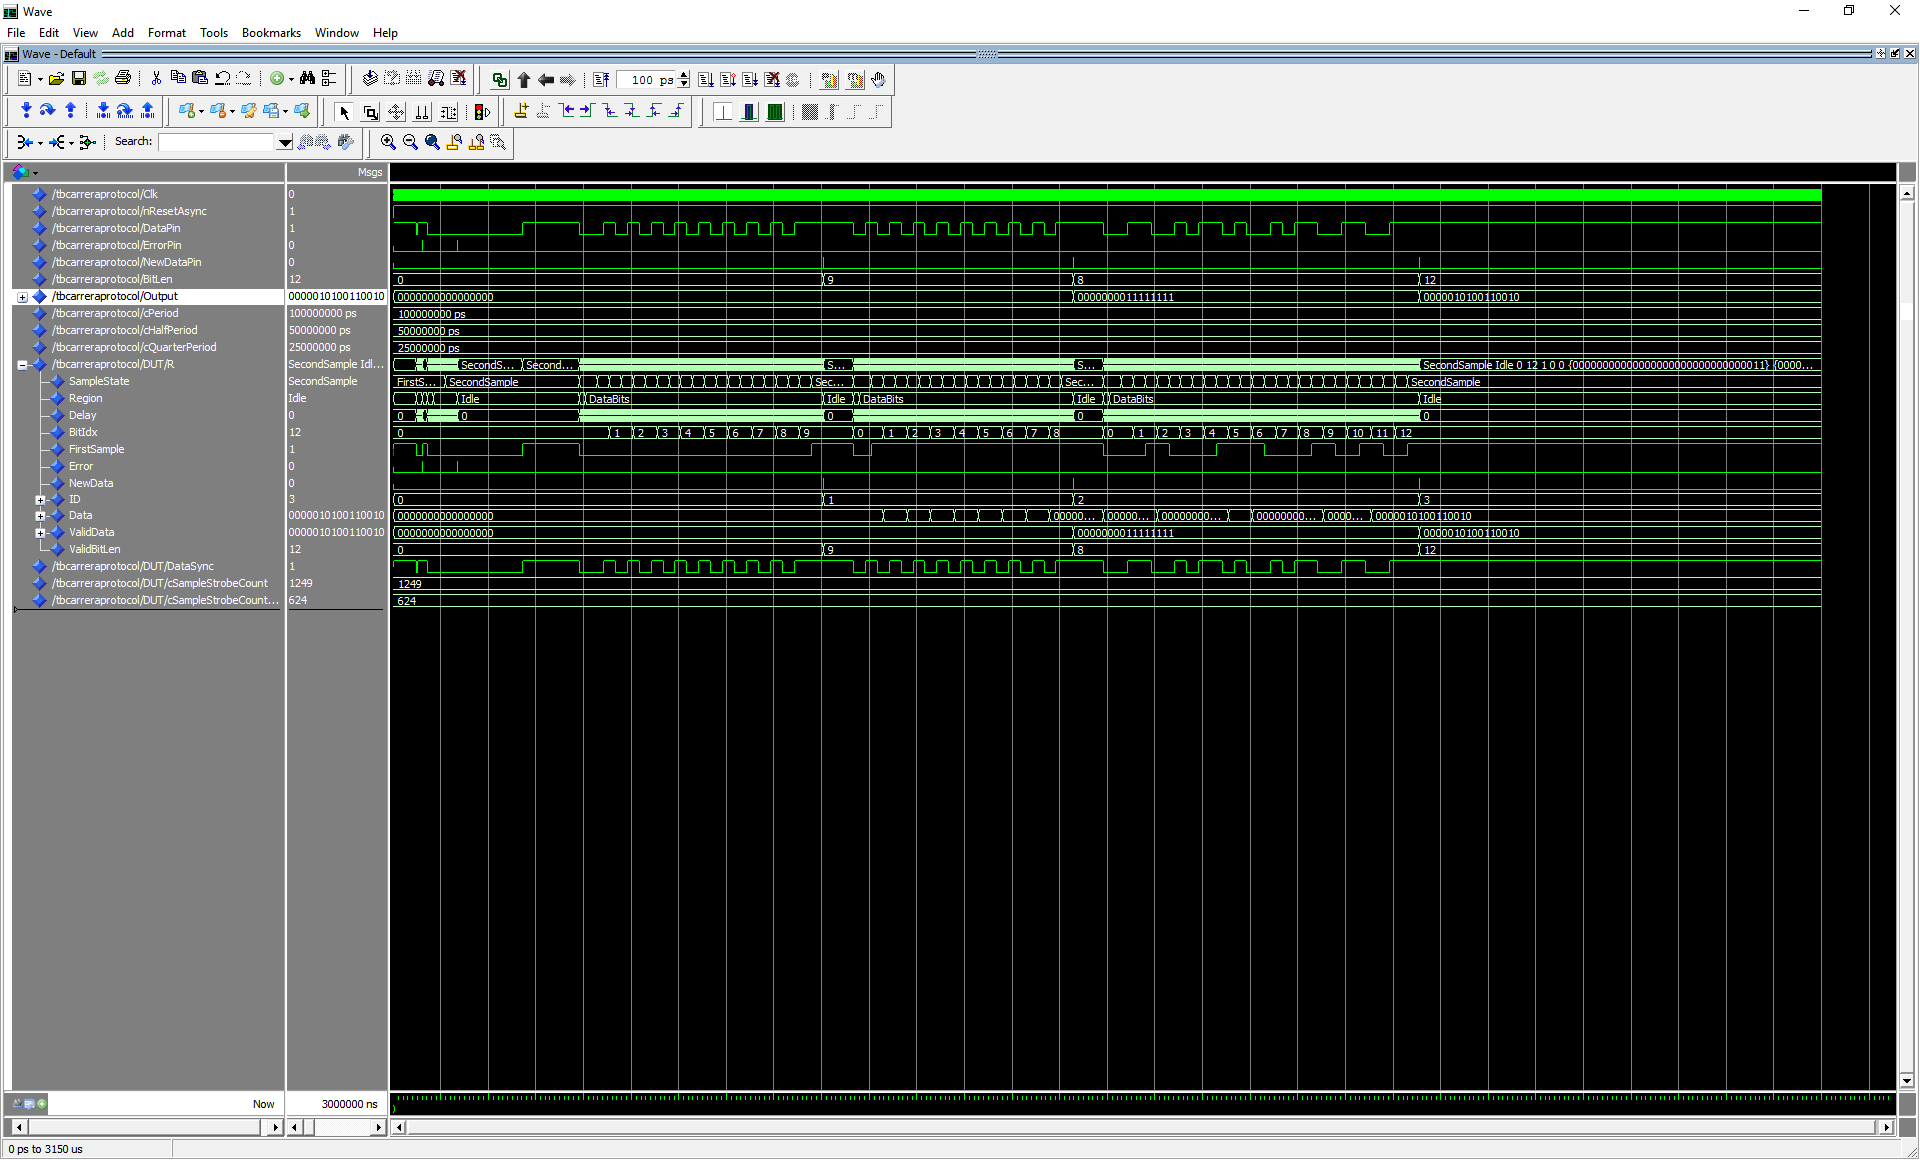
\includegraphics[angle=90,height=1.00\textheight]{./Verification.png}
	\caption{Verification of Carrera Protocol VHDL Design}
	\label{fig:Verification}
\end{figure}





%%%%%%%%%%%%%%%%%%%%%%%%%%%%%%%%%%%%%%%%%%%%%%%%%%
\end {document}

